% Halo models for intrinsic alignments: how each is built, how well it fits
% FLAMINGO, and how much it biases Roman.
% Build with assets/build_note.sh of the summary-notes skill.
\documentclass[11pt]{article}

\usepackage[margin=1in]{geometry}
\usepackage{amsmath}
\usepackage{amssymb}
\usepackage{graphicx}
\usepackage{booktabs}
\usepackage{xcolor}
\usepackage{float}
\usepackage[font=small,labelfont=bf,labelsep=period]{caption}
\usepackage[hidelinks]{hyperref}
% long \texttt paths cannot hyphenate; let the lines stretch instead
\setlength{\emergencystretch}{3em}
% let figures share pages with text
\renewcommand{\topfraction}{0.9}
\renewcommand{\textfraction}{0.07}
\renewcommand{\floatpagefraction}{0.8}

% Symbols, one macro per object.
\newcommand{\hMpc}{\,h\,{\rm Mpc}^{-1}}
\newcommand{\Msun}{\,h^{-1}M_\odot}
\newcommand{\Plin}{P_{\rm lin}}
\newcommand{\PNL}{P_{\rm NL}}
\newcommand{\bTA}{b_{\rm TA}}
\newcommand{\bNL}{\beta_{\rm NL}}
\newcommand{\Cb}{\bar C_1}
\newcommand{\Cbb}{\bar C_2}
\newcommand{\Ib}[1]{I^{\beta}_{#1}}
\newcommand{\dd}{\mathrm{d}}
\newcommand{\kmax}{k_{\max}}

% =====================================================================
% Numbers
% =====================================================================
% Part 1: results, all in numbers.tex, written by make_numbers.py from
% analysis/halo_nlbias/nlbias_fits.json, analysis/halo_nlbias/
% nlbias_roman_tables.npz and plots/fob_k0scan/data.json (which comes from
% analysis/cut_validation/fisher_minimize.json). Every macro there carries
% its source in a comment. Set \numbersfinalfalse to print them in red.
%
% Statements of the text that rest on Part 1 (re-check after a refresh):
%   - the alpha model is the only one with an acceptable FLAMINGO fit to
%     k ~ 1, and beta_NL beats HMc only below k_max ~ 0.5 (sections
%     "Summary", "Goodness of fit on FLAMINGO");
%   - a_c sits at its cap and b_TA drifts in HMc and beta_NL (section
%     "Physical checks");
%   - the Roman bias ordering of the models (section "Figure of bias for Roman").
\newif\ifnumbersfinal
\numbersfinaltrue
\newcommand{\refresh}[1]{\ifnumbersfinal#1\else\textcolor{red}{#1}\fi}
% Written by make_numbers.py; do not edit by hand.
\newcommand{\gofTattBaseA}{5.68}  % nlbias_fits.json tatt: sum chi2 / sum nu at k_max 0.523
\newcommand{\gofTattBaseB}{15.39}  % nlbias_fits.json tatt: sum chi2 / sum nu at k_max 0.701
\newcommand{\gofTattBaseC}{19.39}  % nlbias_fits.json tatt: sum chi2 / sum nu at k_max 0.941
\newcommand{\cutTattBaseLo}{0.29}  % nlbias_fits.json tatt: min GOF cut over z
\newcommand{\cutTattBaseHi}{0.70}  % nlbias_fits.json tatt: max GOF cut over z
\newcommand{\cutTattBaseMed}{0.29}  % nlbias_fits.json tatt: median GOF cut
\newcommand{\acCapTattBaseA}{1}  % nlbias_fits.json tatt: snapshots (of 9) with a_c at its cap 1, k_max 0.523
\newcommand{\aOneTattBaseALo}{3.47}  % tatt: min A1 over z, k_max 0.523
\newcommand{\aOneTattBaseAHi}{5.00}  % tatt: max A1 over z, k_max 0.523
\newcommand{\btaBaseALo}{0.00}  % tatt: min b_TA over z, k_max 0.523
\newcommand{\btaBaseAHi}{0.31}  % tatt: max b_TA over z, k_max 0.523
\newcommand{\acCapTattBaseC}{0}  % nlbias_fits.json tatt: snapshots (of 9) with a_c at its cap 1, k_max 0.941
\newcommand{\aOneTattBaseCLo}{1.83}  % tatt: min A1 over z, k_max 0.941
\newcommand{\aOneTattBaseCHi}{5.60}  % tatt: max A1 over z, k_max 0.941
\newcommand{\btaBaseCLo}{0.00}  % tatt: min b_TA over z, k_max 0.941
\newcommand{\btaBaseCHi}{0.73}  % tatt: max b_TA over z, k_max 0.941
\newcommand{\driftTattBaseLo}{0.55}  % tatt: min A1(0.94)/A1(0.29) over z
\newcommand{\driftTattBaseHi}{1.12}  % tatt: max A1(0.94)/A1(0.29) over z
\newcommand{\gofTattHmcA}{2.10}  % nlbias_fits.json lin_tatt: sum chi2 / sum nu at k_max 0.523
\newcommand{\gofTattHmcB}{4.79}  % nlbias_fits.json lin_tatt: sum chi2 / sum nu at k_max 0.701
\newcommand{\gofTattHmcC}{12.71}  % nlbias_fits.json lin_tatt: sum chi2 / sum nu at k_max 0.941
\newcommand{\cutTattHmcLo}{0.29}  % nlbias_fits.json lin_tatt: min GOF cut over z
\newcommand{\cutTattHmcHi}{0.52}  % nlbias_fits.json lin_tatt: max GOF cut over z
\newcommand{\cutTattHmcMed}{0.39}  % nlbias_fits.json lin_tatt: median GOF cut
\newcommand{\acCapTattHmcA}{9}  % nlbias_fits.json lin_tatt: snapshots (of 9) with a_c at its cap 1, k_max 0.523
\newcommand{\aOneTattHmcALo}{2.80}  % lin_tatt: min A1 over z, k_max 0.523
\newcommand{\aOneTattHmcAHi}{5.17}  % lin_tatt: max A1 over z, k_max 0.523
\newcommand{\btaHmcALo}{0.41}  % lin_tatt: min b_TA over z, k_max 0.523
\newcommand{\btaHmcAHi}{1.24}  % lin_tatt: max b_TA over z, k_max 0.523
\newcommand{\acCapTattHmcC}{9}  % nlbias_fits.json lin_tatt: snapshots (of 9) with a_c at its cap 1, k_max 0.941
\newcommand{\aOneTattHmcCLo}{2.42}  % lin_tatt: min A1 over z, k_max 0.941
\newcommand{\aOneTattHmcCHi}{4.74}  % lin_tatt: max A1 over z, k_max 0.941
\newcommand{\btaHmcCLo}{0.67}  % lin_tatt: min b_TA over z, k_max 0.941
\newcommand{\btaHmcCHi}{1.71}  % lin_tatt: max b_TA over z, k_max 0.941
\newcommand{\driftTattHmcLo}{0.85}  % lin_tatt: min A1(0.94)/A1(0.29) over z
\newcommand{\driftTattHmcHi}{0.95}  % lin_tatt: max A1(0.94)/A1(0.29) over z
\newcommand{\gofTattAlphaA}{0.97}  % nlbias_fits.json alpha_tatt: sum chi2 / sum nu at k_max 0.523
\newcommand{\gofTattAlphaB}{1.08}  % nlbias_fits.json alpha_tatt: sum chi2 / sum nu at k_max 0.701
\newcommand{\gofTattAlphaC}{1.33}  % nlbias_fits.json alpha_tatt: sum chi2 / sum nu at k_max 0.941
\newcommand{\cutTattAlphaLo}{0.70}  % nlbias_fits.json alpha_tatt: min GOF cut over z
\newcommand{\cutTattAlphaHi}{1.69}  % nlbias_fits.json alpha_tatt: max GOF cut over z
\newcommand{\cutTattAlphaMed}{0.94}  % nlbias_fits.json alpha_tatt: median GOF cut
\newcommand{\acCapTattAlphaA}{6}  % nlbias_fits.json alpha_tatt: snapshots (of 9) with a_c at its cap 1, k_max 0.523
\newcommand{\aOneTattAlphaALo}{3.02}  % alpha_tatt: min A1 over z, k_max 0.523
\newcommand{\aOneTattAlphaAHi}{5.30}  % alpha_tatt: max A1 over z, k_max 0.523
\newcommand{\btaAlphaALo}{0.16}  % alpha_tatt: min b_TA over z, k_max 0.523
\newcommand{\btaAlphaAHi}{1.03}  % alpha_tatt: max b_TA over z, k_max 0.523
\newcommand{\alphaTattALo}{0.31}  % alpha_tatt: min alpha over z, k_max 0.523
\newcommand{\alphaTattAHi}{0.76}  % alpha_tatt: max alpha over z, k_max 0.523
\newcommand{\acCapTattAlphaC}{7}  % nlbias_fits.json alpha_tatt: snapshots (of 9) with a_c at its cap 1, k_max 0.941
\newcommand{\aOneTattAlphaCLo}{3.25}  % alpha_tatt: min A1 over z, k_max 0.941
\newcommand{\aOneTattAlphaCHi}{5.46}  % alpha_tatt: max A1 over z, k_max 0.941
\newcommand{\btaAlphaCLo}{0.13}  % alpha_tatt: min b_TA over z, k_max 0.941
\newcommand{\btaAlphaCHi}{0.87}  % alpha_tatt: max b_TA over z, k_max 0.941
\newcommand{\alphaTattCLo}{0.49}  % alpha_tatt: min alpha over z, k_max 0.941
\newcommand{\alphaTattCHi}{0.83}  % alpha_tatt: max alpha over z, k_max 0.941
\newcommand{\driftTattAlphaLo}{1.01}  % alpha_tatt: min A1(0.94)/A1(0.29) over z
\newcommand{\driftTattAlphaHi}{1.08}  % alpha_tatt: max A1(0.94)/A1(0.29) over z
\newcommand{\gofTattNlbA}{1.49}  % nlbias_fits.json nlb_tatt: sum chi2 / sum nu at k_max 0.523
\newcommand{\gofTattNlbB}{4.08}  % nlbias_fits.json nlb_tatt: sum chi2 / sum nu at k_max 0.701
\newcommand{\gofTattNlbC}{15.85}  % nlbias_fits.json nlb_tatt: sum chi2 / sum nu at k_max 0.941
\newcommand{\cutTattNlbLo}{0.22}  % nlbias_fits.json nlb_tatt: min GOF cut over z
\newcommand{\cutTattNlbHi}{0.52}  % nlbias_fits.json nlb_tatt: max GOF cut over z
\newcommand{\cutTattNlbMed}{0.52}  % nlbias_fits.json nlb_tatt: median GOF cut
\newcommand{\acCapTattNlbA}{8}  % nlbias_fits.json nlb_tatt: snapshots (of 9) with a_c at its cap 1, k_max 0.523
\newcommand{\aOneTattNlbALo}{3.05}  % nlb_tatt: min A1 over z, k_max 0.523
\newcommand{\aOneTattNlbAHi}{5.88}  % nlb_tatt: max A1 over z, k_max 0.523
\newcommand{\btaNlbALo}{0.21}  % nlb_tatt: min b_TA over z, k_max 0.523
\newcommand{\btaNlbAHi}{0.38}  % nlb_tatt: max b_TA over z, k_max 0.523
\newcommand{\acCapTattNlbC}{9}  % nlbias_fits.json nlb_tatt: snapshots (of 9) with a_c at its cap 1, k_max 0.941
\newcommand{\aOneTattNlbCLo}{2.54}  % nlb_tatt: min A1 over z, k_max 0.941
\newcommand{\aOneTattNlbCHi}{5.49}  % nlb_tatt: max A1 over z, k_max 0.941
\newcommand{\btaNlbCLo}{0.48}  % nlb_tatt: min b_TA over z, k_max 0.941
\newcommand{\btaNlbCHi}{0.74}  % nlb_tatt: max b_TA over z, k_max 0.941
\newcommand{\driftTattNlbLo}{0.84}  % nlb_tatt: min A1(0.94)/A1(0.29) over z
\newcommand{\driftTattNlbHi}{0.96}  % nlb_tatt: max A1(0.94)/A1(0.29) over z
\newcommand{\gofNlaBaseA}{10.31}  % nlbias_fits.json nla: sum chi2 / sum nu at k_max 0.523
\newcommand{\gofNlaBaseB}{18.66}  % nlbias_fits.json nla: sum chi2 / sum nu at k_max 0.701
\newcommand{\gofNlaBaseC}{26.11}  % nlbias_fits.json nla: sum chi2 / sum nu at k_max 0.941
\newcommand{\cutNlaBaseLo}{0.16}  % nlbias_fits.json nla: min GOF cut over z
\newcommand{\cutNlaBaseHi}{0.39}  % nlbias_fits.json nla: max GOF cut over z
\newcommand{\cutNlaBaseMed}{0.22}  % nlbias_fits.json nla: median GOF cut
\newcommand{\acCapNlaBaseA}{2}  % nlbias_fits.json nla: snapshots (of 9) with a_c at its cap 1, k_max 0.523
\newcommand{\aOneNlaBaseALo}{2.54}  % nla: min A1 over z, k_max 0.523
\newcommand{\aOneNlaBaseAHi}{6.18}  % nla: max A1 over z, k_max 0.523
\newcommand{\acCapNlaBaseC}{2}  % nlbias_fits.json nla: snapshots (of 9) with a_c at its cap 1, k_max 0.941
\newcommand{\aOneNlaBaseCLo}{2.35}  % nla: min A1 over z, k_max 0.941
\newcommand{\aOneNlaBaseCHi}{6.70}  % nla: max A1 over z, k_max 0.941
\newcommand{\driftNlaBaseLo}{0.83}  % nla: min A1(0.94)/A1(0.29) over z
\newcommand{\driftNlaBaseHi}{1.15}  % nla: max A1(0.94)/A1(0.29) over z
\newcommand{\gofNlaHmcA}{88.82}  % nlbias_fits.json lin_nla: sum chi2 / sum nu at k_max 0.523
\newcommand{\gofNlaHmcB}{242.92}  % nlbias_fits.json lin_nla: sum chi2 / sum nu at k_max 0.701
\newcommand{\gofNlaHmcC}{602.96}  % nlbias_fits.json lin_nla: sum chi2 / sum nu at k_max 0.941
\newcommand{\cutNlaHmcLo}{0.12}  % nlbias_fits.json lin_nla: min GOF cut over z
\newcommand{\cutNlaHmcHi}{0.16}  % nlbias_fits.json lin_nla: max GOF cut over z
\newcommand{\cutNlaHmcMed}{0.16}  % nlbias_fits.json lin_nla: median GOF cut
\newcommand{\acCapNlaHmcA}{9}  % nlbias_fits.json lin_nla: snapshots (of 9) with a_c at its cap 1, k_max 0.523
\newcommand{\aOneNlaHmcALo}{3.90}  % lin_nla: min A1 over z, k_max 0.523
\newcommand{\aOneNlaHmcAHi}{7.07}  % lin_nla: max A1 over z, k_max 0.523
\newcommand{\acCapNlaHmcC}{9}  % nlbias_fits.json lin_nla: snapshots (of 9) with a_c at its cap 1, k_max 0.941
\newcommand{\aOneNlaHmcCLo}{4.87}  % lin_nla: min A1 over z, k_max 0.941
\newcommand{\aOneNlaHmcCHi}{8.66}  % lin_nla: max A1 over z, k_max 0.941
\newcommand{\driftNlaHmcLo}{1.40}  % lin_nla: min A1(0.94)/A1(0.29) over z
\newcommand{\driftNlaHmcHi}{1.46}  % lin_nla: max A1(0.94)/A1(0.29) over z
\newcommand{\gofNlaAlphaA}{1.77}  % nlbias_fits.json alpha_nla: sum chi2 / sum nu at k_max 0.523
\newcommand{\gofNlaAlphaB}{2.58}  % nlbias_fits.json alpha_nla: sum chi2 / sum nu at k_max 0.701
\newcommand{\gofNlaAlphaC}{3.94}  % nlbias_fits.json alpha_nla: sum chi2 / sum nu at k_max 0.941
\newcommand{\cutNlaAlphaLo}{0.22}  % nlbias_fits.json alpha_nla: min GOF cut over z
\newcommand{\cutNlaAlphaHi}{0.70}  % nlbias_fits.json alpha_nla: max GOF cut over z
\newcommand{\cutNlaAlphaMed}{0.39}  % nlbias_fits.json alpha_nla: median GOF cut
\newcommand{\acCapNlaAlphaA}{1}  % nlbias_fits.json alpha_nla: snapshots (of 9) with a_c at its cap 1, k_max 0.523
\newcommand{\aOneNlaAlphaALo}{3.05}  % alpha_nla: min A1 over z, k_max 0.523
\newcommand{\aOneNlaAlphaAHi}{5.65}  % alpha_nla: max A1 over z, k_max 0.523
\newcommand{\alphaNlaALo}{0.58}  % alpha_nla: min alpha over z, k_max 0.523
\newcommand{\alphaNlaAHi}{1.65}  % alpha_nla: max alpha over z, k_max 0.523
\newcommand{\acCapNlaAlphaC}{5}  % nlbias_fits.json alpha_nla: snapshots (of 9) with a_c at its cap 1, k_max 0.941
\newcommand{\aOneNlaAlphaCLo}{2.99}  % alpha_nla: min A1 over z, k_max 0.941
\newcommand{\aOneNlaAlphaCHi}{5.79}  % alpha_nla: max A1 over z, k_max 0.941
\newcommand{\alphaNlaCLo}{0.64}  % alpha_nla: min alpha over z, k_max 0.941
\newcommand{\alphaNlaCHi}{1.53}  % alpha_nla: max alpha over z, k_max 0.941
\newcommand{\driftNlaAlphaLo}{1.00}  % alpha_nla: min A1(0.94)/A1(0.29) over z
\newcommand{\driftNlaAlphaHi}{1.04}  % alpha_nla: max A1(0.94)/A1(0.29) over z
\newcommand{\gofNlaNlbA}{9.84}  % nlbias_fits.json nlb_nla: sum chi2 / sum nu at k_max 0.523
\newcommand{\gofNlaNlbB}{40.16}  % nlbias_fits.json nlb_nla: sum chi2 / sum nu at k_max 0.701
\newcommand{\gofNlaNlbC}{157.21}  % nlbias_fits.json nlb_nla: sum chi2 / sum nu at k_max 0.941
\newcommand{\cutNlaNlbLo}{0.22}  % nlbias_fits.json nlb_nla: min GOF cut over z
\newcommand{\cutNlaNlbHi}{0.39}  % nlbias_fits.json nlb_nla: max GOF cut over z
\newcommand{\cutNlaNlbMed}{0.29}  % nlbias_fits.json nlb_nla: median GOF cut
\newcommand{\acCapNlaNlbA}{9}  % nlbias_fits.json nlb_nla: snapshots (of 9) with a_c at its cap 1, k_max 0.523
\newcommand{\aOneNlaNlbALo}{3.56}  % nlb_nla: min A1 over z, k_max 0.523
\newcommand{\aOneNlaNlbAHi}{5.82}  % nlb_nla: max A1 over z, k_max 0.523
\newcommand{\acCapNlaNlbC}{9}  % nlbias_fits.json nlb_nla: snapshots (of 9) with a_c at its cap 1, k_max 0.941
\newcommand{\aOneNlaNlbCLo}{4.32}  % nlb_nla: min A1 over z, k_max 0.941
\newcommand{\aOneNlaNlbCHi}{6.33}  % nlb_nla: max A1 over z, k_max 0.941
\newcommand{\driftNlaNlbLo}{1.10}  % nlb_nla: min A1(0.94)/A1(0.29) over z
\newcommand{\driftNlaNlbHi}{1.32}  % nlb_nla: max A1(0.94)/A1(0.29) over z
\newcommand{\lowkSpreadTattLo}{4}  % TATT form: min over z of max |A1/mean - 1| [%] at k_max 0.291
\newcommand{\lowkSpreadTattHi}{11}  % TATT form: max over z of max |A1/mean - 1| [%] at k_max 0.291
\newcommand{\lowkSpreadNlaLo}{6}  % NLA form: min over z of max |A1/mean - 1| [%] at k_max 0.291
\newcommand{\lowkSpreadNlaHi}{10}  % NLA form: max over z of max |A1/mean - 1| [%] at k_max 0.291
\newcommand{\ibcmA}{-0.03}  % nlbias_roman_tables.npz Ib_cm, z = 1, k = 0.102
\newcommand{\ibcmLoA}{-0.00}  % nlbias_roman_tables.npz Ib_cm_lo, z = 1, k = 0.102
\newcommand{\ibcmB}{0.18}  % nlbias_roman_tables.npz Ib_cm, z = 1, k = 0.295
\newcommand{\ibcmLoB}{0.01}  % nlbias_roman_tables.npz Ib_cm_lo, z = 1, k = 0.295
\newcommand{\ibcmC}{0.44}  % nlbias_roman_tables.npz Ib_cm, z = 1, k = 0.490
\newcommand{\ibcmLoC}{0.01}  % nlbias_roman_tables.npz Ib_cm_lo, z = 1, k = 0.490
\newcommand{\ibcmD}{0.95}  % nlbias_roman_tables.npz Ib_cm, z = 1, k = 0.978
\newcommand{\ibcmLoD}{0.02}  % nlbias_roman_tables.npz Ib_cm_lo, z = 1, k = 0.978
\newcommand{\dipLo}{-0.05}  % Ib_cm, z = 0.2 to 2, 0.05 < k < 0.15: min
\newcommand{\dipHi}{0.00}  % Ib_cm, z = 0.2 to 2, 0.05 < k < 0.15: max
\newcommand{\lgMElo}{11.9}  % nlbias_roman_tables.npz lgM_E: lowest emulator mass, z = 0.2 to 2
\newcommand{\lgMEhi}{12.7}  % nlbias_roman_tables.npz lgM_E: lowest emulator mass, z = 0.2 to 2
\newcommand{\fobCsTattBase}{0.18}  % fob_k0scan/data.json cs|TATT|base at K0 = 0.35
\newcommand{\ctwoCsTattBase}{1.9}  % fob_k0scan/data.json cs|TATT|base: chi2 of the IA reference fit at K0 = 0.35
\newcommand{\ctwoTopCsTattBase}{3.2}  % fob_k0scan/data.json cs|TATT|base: chi2 of the IA reference fit at K0 = 0.6
\newcommand{\fobTopCsTattBase}{0.27}  % fob_k0scan/data.json cs|TATT|base at K0 = 0.6
\newcommand{\fobMaxCsTattBase}{0.27}  % fob_k0scan/data.json cs|TATT|base: max over K0
\newcommand{\kmaxCsTattBase}{0.6}  % fob_k0scan/data.json cs|TATT|base: largest K0 with FoB < 0.3 at every smaller K0
\newcommand{\bndCsTattBase}{A2\_2, BTA\_1}  % fob_k0scan/data.json cs|TATT|base: reference parameters at a bound, any K0
\newcommand{\fobCsTattHmc}{0.28}  % fob_k0scan/data.json cs|TATT|hmc at K0 = 0.35
\newcommand{\ctwoCsTattHmc}{2.2}  % fob_k0scan/data.json cs|TATT|hmc: chi2 of the IA reference fit at K0 = 0.35
\newcommand{\ctwoTopCsTattHmc}{4.6}  % fob_k0scan/data.json cs|TATT|hmc: chi2 of the IA reference fit at K0 = 0.6
\newcommand{\fobTopCsTattHmc}{0.43}  % fob_k0scan/data.json cs|TATT|hmc at K0 = 0.6
\newcommand{\fobMaxCsTattHmc}{0.43}  % fob_k0scan/data.json cs|TATT|hmc: max over K0
\newcommand{\kmaxCsTattHmc}{0.4}  % fob_k0scan/data.json cs|TATT|hmc: largest K0 with FoB < 0.3 at every smaller K0
\newcommand{\bndCsTattHmc}{none}  % fob_k0scan/data.json cs|TATT|hmc: reference parameters at a bound, any K0
\newcommand{\fobCsTattAlpha}{0.18}  % fob_k0scan/data.json cs|TATT|alpha at K0 = 0.35
\newcommand{\ctwoCsTattAlpha}{1.9}  % fob_k0scan/data.json cs|TATT|alpha: chi2 of the IA reference fit at K0 = 0.35
\newcommand{\ctwoTopCsTattAlpha}{3.5}  % fob_k0scan/data.json cs|TATT|alpha: chi2 of the IA reference fit at K0 = 0.6
\newcommand{\fobTopCsTattAlpha}{0.25}  % fob_k0scan/data.json cs|TATT|alpha at K0 = 0.6
\newcommand{\fobMaxCsTattAlpha}{0.25}  % fob_k0scan/data.json cs|TATT|alpha: max over K0
\newcommand{\kmaxCsTattAlpha}{0.6}  % fob_k0scan/data.json cs|TATT|alpha: largest K0 with FoB < 0.3 at every smaller K0
\newcommand{\bndCsTattAlpha}{none}  % fob_k0scan/data.json cs|TATT|alpha: reference parameters at a bound, any K0
\newcommand{\fobCsTattAlphaf}{0.22}  % fob_k0scan/data.json cs|TATT|alphaf at K0 = 0.35
\newcommand{\ctwoCsTattAlphaf}{1.9}  % fob_k0scan/data.json cs|TATT|alphaf: chi2 of the IA reference fit at K0 = 0.35
\newcommand{\ctwoTopCsTattAlphaf}{3.6}  % fob_k0scan/data.json cs|TATT|alphaf: chi2 of the IA reference fit at K0 = 0.6
\newcommand{\fobTopCsTattAlphaf}{0.31}  % fob_k0scan/data.json cs|TATT|alphaf at K0 = 0.6
\newcommand{\fobMaxCsTattAlphaf}{0.31}  % fob_k0scan/data.json cs|TATT|alphaf: max over K0
\newcommand{\kmaxCsTattAlphaf}{0.5}  % fob_k0scan/data.json cs|TATT|alphaf: largest K0 with FoB < 0.3 at every smaller K0
\newcommand{\bndCsTattAlphaf}{none}  % fob_k0scan/data.json cs|TATT|alphaf: reference parameters at a bound, any K0
\newcommand{\fobCsTattNlb}{0.15}  % fob_k0scan/data.json cs|TATT|nlb at K0 = 0.35
\newcommand{\ctwoCsTattNlb}{2.1}  % fob_k0scan/data.json cs|TATT|nlb: chi2 of the IA reference fit at K0 = 0.35
\newcommand{\ctwoTopCsTattNlb}{3.0}  % fob_k0scan/data.json cs|TATT|nlb: chi2 of the IA reference fit at K0 = 0.6
\newcommand{\fobTopCsTattNlb}{0.20}  % fob_k0scan/data.json cs|TATT|nlb at K0 = 0.6
\newcommand{\fobMaxCsTattNlb}{0.20}  % fob_k0scan/data.json cs|TATT|nlb: max over K0
\newcommand{\kmaxCsTattNlb}{0.6}  % fob_k0scan/data.json cs|TATT|nlb: largest K0 with FoB < 0.3 at every smaller K0
\newcommand{\bndCsTattNlb}{A2\_2, BTA\_1}  % fob_k0scan/data.json cs|TATT|nlb: reference parameters at a bound, any K0
\newcommand{\fobCsNlaBase}{0.19}  % fob_k0scan/data.json cs|NLA|base at K0 = 0.35
\newcommand{\ctwoCsNlaBase}{1.9}  % fob_k0scan/data.json cs|NLA|base: chi2 of the IA reference fit at K0 = 0.35
\newcommand{\ctwoTopCsNlaBase}{3.8}  % fob_k0scan/data.json cs|NLA|base: chi2 of the IA reference fit at K0 = 0.6
\newcommand{\fobTopCsNlaBase}{0.24}  % fob_k0scan/data.json cs|NLA|base at K0 = 0.6
\newcommand{\fobMaxCsNlaBase}{0.24}  % fob_k0scan/data.json cs|NLA|base: max over K0
\newcommand{\kmaxCsNlaBase}{0.6}  % fob_k0scan/data.json cs|NLA|base: largest K0 with FoB < 0.3 at every smaller K0
\newcommand{\bndCsNlaBase}{none}  % fob_k0scan/data.json cs|NLA|base: reference parameters at a bound, any K0
\newcommand{\fobCsNlaHmc}{0.14}  % fob_k0scan/data.json cs|NLA|hmc at K0 = 0.35
\newcommand{\ctwoCsNlaHmc}{2.7}  % fob_k0scan/data.json cs|NLA|hmc: chi2 of the IA reference fit at K0 = 0.35
\newcommand{\ctwoTopCsNlaHmc}{8.8}  % fob_k0scan/data.json cs|NLA|hmc: chi2 of the IA reference fit at K0 = 0.6
\newcommand{\fobTopCsNlaHmc}{0.22}  % fob_k0scan/data.json cs|NLA|hmc at K0 = 0.6
\newcommand{\fobMaxCsNlaHmc}{0.22}  % fob_k0scan/data.json cs|NLA|hmc: max over K0
\newcommand{\kmaxCsNlaHmc}{0.6}  % fob_k0scan/data.json cs|NLA|hmc: largest K0 with FoB < 0.3 at every smaller K0
\newcommand{\bndCsNlaHmc}{none}  % fob_k0scan/data.json cs|NLA|hmc: reference parameters at a bound, any K0
\newcommand{\fobCsNlaAlpha}{0.20}  % fob_k0scan/data.json cs|NLA|alpha at K0 = 0.35
\newcommand{\ctwoCsNlaAlpha}{1.9}  % fob_k0scan/data.json cs|NLA|alpha: chi2 of the IA reference fit at K0 = 0.35
\newcommand{\ctwoTopCsNlaAlpha}{3.7}  % fob_k0scan/data.json cs|NLA|alpha: chi2 of the IA reference fit at K0 = 0.6
\newcommand{\fobTopCsNlaAlpha}{0.26}  % fob_k0scan/data.json cs|NLA|alpha at K0 = 0.6
\newcommand{\fobMaxCsNlaAlpha}{0.26}  % fob_k0scan/data.json cs|NLA|alpha: max over K0
\newcommand{\kmaxCsNlaAlpha}{0.6}  % fob_k0scan/data.json cs|NLA|alpha: largest K0 with FoB < 0.3 at every smaller K0
\newcommand{\bndCsNlaAlpha}{none}  % fob_k0scan/data.json cs|NLA|alpha: reference parameters at a bound, any K0
\newcommand{\fobCsNlaAlphaf}{0.18}  % fob_k0scan/data.json cs|NLA|alphaf at K0 = 0.35
\newcommand{\ctwoCsNlaAlphaf}{1.9}  % fob_k0scan/data.json cs|NLA|alphaf: chi2 of the IA reference fit at K0 = 0.35
\newcommand{\ctwoTopCsNlaAlphaf}{4.1}  % fob_k0scan/data.json cs|NLA|alphaf: chi2 of the IA reference fit at K0 = 0.6
\newcommand{\fobTopCsNlaAlphaf}{0.27}  % fob_k0scan/data.json cs|NLA|alphaf at K0 = 0.6
\newcommand{\fobMaxCsNlaAlphaf}{0.27}  % fob_k0scan/data.json cs|NLA|alphaf: max over K0
\newcommand{\kmaxCsNlaAlphaf}{0.6}  % fob_k0scan/data.json cs|NLA|alphaf: largest K0 with FoB < 0.3 at every smaller K0
\newcommand{\bndCsNlaAlphaf}{none}  % fob_k0scan/data.json cs|NLA|alphaf: reference parameters at a bound, any K0
\newcommand{\fobCsNlaNlb}{0.30}  % fob_k0scan/data.json cs|NLA|nlb at K0 = 0.35
\newcommand{\ctwoCsNlaNlb}{2.5}  % fob_k0scan/data.json cs|NLA|nlb: chi2 of the IA reference fit at K0 = 0.35
\newcommand{\ctwoTopCsNlaNlb}{5.5}  % fob_k0scan/data.json cs|NLA|nlb: chi2 of the IA reference fit at K0 = 0.6
\newcommand{\fobTopCsNlaNlb}{0.64}  % fob_k0scan/data.json cs|NLA|nlb at K0 = 0.6
\newcommand{\fobMaxCsNlaNlb}{0.64}  % fob_k0scan/data.json cs|NLA|nlb: max over K0
\newcommand{\kmaxCsNlaNlb}{0.3}  % fob_k0scan/data.json cs|NLA|nlb: largest K0 with FoB < 0.3 at every smaller K0
\newcommand{\bndCsNlaNlb}{none}  % fob_k0scan/data.json cs|NLA|nlb: reference parameters at a bound, any K0
\newcommand{\fobTxTattBase}{0.17}  % fob_k0scan/data.json 3x2|TATT|base at K0 = 0.2
\newcommand{\ctwoTxTattBase}{1.2}  % fob_k0scan/data.json 3x2|TATT|base: chi2 of the IA reference fit at K0 = 0.2
\newcommand{\ctwoTopTxTattBase}{3.6}  % fob_k0scan/data.json 3x2|TATT|base: chi2 of the IA reference fit at K0 = 0.6
\newcommand{\fobTopTxTattBase}{0.44}  % fob_k0scan/data.json 3x2|TATT|base at K0 = 0.6
\newcommand{\fobMaxTxTattBase}{0.44}  % fob_k0scan/data.json 3x2|TATT|base: max over K0
\newcommand{\kmaxTxTattBase}{0.35}  % fob_k0scan/data.json 3x2|TATT|base: largest K0 with FoB < 0.3 at every smaller K0
\newcommand{\bndTxTattBase}{A2\_2, BTA\_1}  % fob_k0scan/data.json 3x2|TATT|base: reference parameters at a bound, any K0
\newcommand{\fobTxTattHmc}{0.19}  % fob_k0scan/data.json 3x2|TATT|hmc at K0 = 0.2
\newcommand{\ctwoTxTattHmc}{1.3}  % fob_k0scan/data.json 3x2|TATT|hmc: chi2 of the IA reference fit at K0 = 0.2
\newcommand{\ctwoTopTxTattHmc}{4.9}  % fob_k0scan/data.json 3x2|TATT|hmc: chi2 of the IA reference fit at K0 = 0.6
\newcommand{\fobTopTxTattHmc}{0.39}  % fob_k0scan/data.json 3x2|TATT|hmc at K0 = 0.6
\newcommand{\fobMaxTxTattHmc}{0.39}  % fob_k0scan/data.json 3x2|TATT|hmc: max over K0
\newcommand{\kmaxTxTattHmc}{0.35}  % fob_k0scan/data.json 3x2|TATT|hmc: largest K0 with FoB < 0.3 at every smaller K0
\newcommand{\bndTxTattHmc}{none}  % fob_k0scan/data.json 3x2|TATT|hmc: reference parameters at a bound, any K0
\newcommand{\fobTxTattAlpha}{0.18}  % fob_k0scan/data.json 3x2|TATT|alpha at K0 = 0.2
\newcommand{\ctwoTxTattAlpha}{1.2}  % fob_k0scan/data.json 3x2|TATT|alpha: chi2 of the IA reference fit at K0 = 0.2
\newcommand{\ctwoTopTxTattAlpha}{4.2}  % fob_k0scan/data.json 3x2|TATT|alpha: chi2 of the IA reference fit at K0 = 0.6
\newcommand{\fobTopTxTattAlpha}{0.48}  % fob_k0scan/data.json 3x2|TATT|alpha at K0 = 0.6
\newcommand{\fobMaxTxTattAlpha}{0.48}  % fob_k0scan/data.json 3x2|TATT|alpha: max over K0
\newcommand{\kmaxTxTattAlpha}{0.35}  % fob_k0scan/data.json 3x2|TATT|alpha: largest K0 with FoB < 0.3 at every smaller K0
\newcommand{\bndTxTattAlpha}{A2\_2}  % fob_k0scan/data.json 3x2|TATT|alpha: reference parameters at a bound, any K0
\newcommand{\fobTxTattAlphaf}{0.18}  % fob_k0scan/data.json 3x2|TATT|alphaf at K0 = 0.2
\newcommand{\ctwoTxTattAlphaf}{1.2}  % fob_k0scan/data.json 3x2|TATT|alphaf: chi2 of the IA reference fit at K0 = 0.2
\newcommand{\ctwoTopTxTattAlphaf}{4.1}  % fob_k0scan/data.json 3x2|TATT|alphaf: chi2 of the IA reference fit at K0 = 0.6
\newcommand{\fobTopTxTattAlphaf}{0.48}  % fob_k0scan/data.json 3x2|TATT|alphaf at K0 = 0.6
\newcommand{\fobMaxTxTattAlphaf}{0.48}  % fob_k0scan/data.json 3x2|TATT|alphaf: max over K0
\newcommand{\kmaxTxTattAlphaf}{0.35}  % fob_k0scan/data.json 3x2|TATT|alphaf: largest K0 with FoB < 0.3 at every smaller K0
\newcommand{\bndTxTattAlphaf}{none}  % fob_k0scan/data.json 3x2|TATT|alphaf: reference parameters at a bound, any K0
\newcommand{\fobTxTattNlb}{0.10}  % fob_k0scan/data.json 3x2|TATT|nlb at K0 = 0.2
\newcommand{\ctwoTxTattNlb}{1.8}  % fob_k0scan/data.json 3x2|TATT|nlb: chi2 of the IA reference fit at K0 = 0.2
\newcommand{\ctwoTopTxTattNlb}{3.6}  % fob_k0scan/data.json 3x2|TATT|nlb: chi2 of the IA reference fit at K0 = 0.6
\newcommand{\fobTopTxTattNlb}{0.41}  % fob_k0scan/data.json 3x2|TATT|nlb at K0 = 0.6
\newcommand{\fobMaxTxTattNlb}{0.41}  % fob_k0scan/data.json 3x2|TATT|nlb: max over K0
\newcommand{\kmaxTxTattNlb}{0.35}  % fob_k0scan/data.json 3x2|TATT|nlb: largest K0 with FoB < 0.3 at every smaller K0
\newcommand{\bndTxTattNlb}{A2\_2, BTA\_1}  % fob_k0scan/data.json 3x2|TATT|nlb: reference parameters at a bound, any K0
\newcommand{\fobTxNlaBase}{0.26}  % fob_k0scan/data.json 3x2|NLA|base at K0 = 0.2
\newcommand{\ctwoTxNlaBase}{1.7}  % fob_k0scan/data.json 3x2|NLA|base: chi2 of the IA reference fit at K0 = 0.2
\newcommand{\ctwoTopTxNlaBase}{4.7}  % fob_k0scan/data.json 3x2|NLA|base: chi2 of the IA reference fit at K0 = 0.6
\newcommand{\fobTopTxNlaBase}{0.49}  % fob_k0scan/data.json 3x2|NLA|base at K0 = 0.6
\newcommand{\fobMaxTxNlaBase}{0.49}  % fob_k0scan/data.json 3x2|NLA|base: max over K0
\newcommand{\kmaxTxNlaBase}{0.25}  % fob_k0scan/data.json 3x2|NLA|base: largest K0 with FoB < 0.3 at every smaller K0
\newcommand{\bndTxNlaBase}{none}  % fob_k0scan/data.json 3x2|NLA|base: reference parameters at a bound, any K0
\newcommand{\fobTxNlaHmc}{0.13}  % fob_k0scan/data.json 3x2|NLA|hmc at K0 = 0.2
\newcommand{\ctwoTxNlaHmc}{2.7}  % fob_k0scan/data.json 3x2|NLA|hmc: chi2 of the IA reference fit at K0 = 0.2
\newcommand{\ctwoTopTxNlaHmc}{12.3}  % fob_k0scan/data.json 3x2|NLA|hmc: chi2 of the IA reference fit at K0 = 0.6
\newcommand{\fobTopTxNlaHmc}{0.20}  % fob_k0scan/data.json 3x2|NLA|hmc at K0 = 0.6
\newcommand{\fobMaxTxNlaHmc}{0.20}  % fob_k0scan/data.json 3x2|NLA|hmc: max over K0
\newcommand{\kmaxTxNlaHmc}{0.6}  % fob_k0scan/data.json 3x2|NLA|hmc: largest K0 with FoB < 0.3 at every smaller K0
\newcommand{\bndTxNlaHmc}{none}  % fob_k0scan/data.json 3x2|NLA|hmc: reference parameters at a bound, any K0
\newcommand{\fobTxNlaAlpha}{0.25}  % fob_k0scan/data.json 3x2|NLA|alpha at K0 = 0.2
\newcommand{\ctwoTxNlaAlpha}{1.7}  % fob_k0scan/data.json 3x2|NLA|alpha: chi2 of the IA reference fit at K0 = 0.2
\newcommand{\ctwoTopTxNlaAlpha}{4.6}  % fob_k0scan/data.json 3x2|NLA|alpha: chi2 of the IA reference fit at K0 = 0.6
\newcommand{\fobTopTxNlaAlpha}{0.51}  % fob_k0scan/data.json 3x2|NLA|alpha at K0 = 0.6
\newcommand{\fobMaxTxNlaAlpha}{0.51}  % fob_k0scan/data.json 3x2|NLA|alpha: max over K0
\newcommand{\kmaxTxNlaAlpha}{0.25}  % fob_k0scan/data.json 3x2|NLA|alpha: largest K0 with FoB < 0.3 at every smaller K0
\newcommand{\bndTxNlaAlpha}{none}  % fob_k0scan/data.json 3x2|NLA|alpha: reference parameters at a bound, any K0
\newcommand{\fobTxNlaAlphaf}{0.29}  % fob_k0scan/data.json 3x2|NLA|alphaf at K0 = 0.2
\newcommand{\ctwoTxNlaAlphaf}{1.9}  % fob_k0scan/data.json 3x2|NLA|alphaf: chi2 of the IA reference fit at K0 = 0.2
\newcommand{\ctwoTopTxNlaAlphaf}{5.1}  % fob_k0scan/data.json 3x2|NLA|alphaf: chi2 of the IA reference fit at K0 = 0.6
\newcommand{\fobTopTxNlaAlphaf}{0.46}  % fob_k0scan/data.json 3x2|NLA|alphaf at K0 = 0.6
\newcommand{\fobMaxTxNlaAlphaf}{0.46}  % fob_k0scan/data.json 3x2|NLA|alphaf: max over K0
\newcommand{\kmaxTxNlaAlphaf}{0.2}  % fob_k0scan/data.json 3x2|NLA|alphaf: largest K0 with FoB < 0.3 at every smaller K0
\newcommand{\bndTxNlaAlphaf}{none}  % fob_k0scan/data.json 3x2|NLA|alphaf: reference parameters at a bound, any K0
\newcommand{\fobTxNlaNlb}{0.19}  % fob_k0scan/data.json 3x2|NLA|nlb at K0 = 0.2
\newcommand{\ctwoTxNlaNlb}{2.9}  % fob_k0scan/data.json 3x2|NLA|nlb: chi2 of the IA reference fit at K0 = 0.2
\newcommand{\ctwoTopTxNlaNlb}{7.3}  % fob_k0scan/data.json 3x2|NLA|nlb: chi2 of the IA reference fit at K0 = 0.6
\newcommand{\fobTopTxNlaNlb}{0.37}  % fob_k0scan/data.json 3x2|NLA|nlb at K0 = 0.6
\newcommand{\fobMaxTxNlaNlb}{0.37}  % fob_k0scan/data.json 3x2|NLA|nlb: max over K0
\newcommand{\kmaxTxNlaNlb}{0.35}  % fob_k0scan/data.json 3x2|NLA|nlb: largest K0 with FoB < 0.3 at every smaller K0
\newcommand{\bndTxNlaNlb}{none}  % fob_k0scan/data.json 3x2|NLA|nlb: reference parameters at a bound, any K0

% Part 2: inputs, which a rerun does not change.
\newcommand{\Kmin}{0.05}           % lowest k of the FLAMINGO fits [h/Mpc] (hmc_alpha_fit.KMIN)
\newcommand{\Ktwoh}{6}             % f_2h = exp[-(k/6)^2] (hmc_alpha_fit.K2H)
\newcommand{\NsnapCore}{9}         % core FLAMINGO snapshots, z = 0.2 to 2
\newcommand{\Nsnap}{13}            % snapshots of the Roman IA base, z = 0 to 4
\newcommand{\ZEmu}{1.48}           % highest redshift of Dark Emulator
\newcommand{\GtCut}{0.5}           % gamma_t cut of the 3x2pt FoB [h/Mpc]
\newcommand{\WCut}{0.2}            % w cut of the 3x2pt FoB [h/Mpc]

\begin{document}

\begin{center}
  {\LARGE Halo models for intrinsic alignments\par}
  \vspace{0.6em}
  {\large How each model is built, how well it fits FLAMINGO, and how much it biases Roman\par}
  \vspace{0.6em}
  {\large November 2026\par}
  \ifnumbersfinal\else
    \vspace{0.6em}
    {\color{red}Numbers in red are being refreshed.\par}
  \fi
\end{center}
\vspace{1em}

\section{Summary}
\label{sec:summary}

\paragraph{The question.}
Which halo model of intrinsic alignments (IA) describes the FLAMINGO IA
spectra to $k \sim 1\hMpc$ with physical parameters, and does using it
lower the bias of Roman's $(\Omega_m, S_8)$?

\paragraph{The answer.}
None of the three physical halo models does. The halo model with a central
1-halo term (HMc) and its extension with nonlinear halo bias $\bNL$ (Mead \&
Verde 2021, arXiv:2011.08858) both fail the goodness of fit beyond
$\kmax \approx 0.5\hMpc$ (summed $\chi^2/\nu$ at $\kmax = 0.52$, 0.70, 0.94:
HMc \gofTattHmcA, \gofTattHmcB, \gofTattHmcC; $\bNL$ \gofTattNlbA,
\gofTattNlbB, \gofTattNlbC). Both keep their central 1-halo amplitude at its
physical cap, and their $\bTA$ drifts with the fit range. Only the
phenomenological model that adds a free share $\alpha$ of $\PNL$ to the
2-halo term fits to $\kmax \approx 1$ (\gofTattAlphaA, \gofTattAlphaB,
\gofTattAlphaC; goodness-of-fit cuts \cutTattAlphaLo\ to
\cutTattAlphaHi$\hMpc$). For Roman, with every parameter free and the CMB
prior, the TATT-form cuts do not move with any halo model: in cosmic shear the
figure of bias (FoB) stays below 0.3 to $K_0 = \kmaxCsTattBase$ for TATT,
$\alpha$ free and $\bNL$, and only to \kmaxCsTattHmc\ for HMc; in 3x2pt to
\kmaxTxTattBase\ for all. $\bNL$ in the TATT form is the least biased model in
cosmic shear from $K_0 = 0.25$ on (\fobCsTattNlb\ against \fobCsTattBase\ for TATT at
$K_0 = 0.35$). The $\alpha$ models follow NLA and TATT within 0.05. In the NLA
form, $\bNL$ is far more biased in cosmic shear (cut \kmaxCsNlaNlb\ against
\kmaxCsNlaBase), and HMc is the least biased model in 3x2pt only because
its errors cancel: its reference $\chi^2$ is 2 to 3 times NLA's, and it is
the worst fit to FLAMINGO (section ``Figure of bias for Roman'').

\paragraph{Why.}
Below $k \approx 1$ the IA signal is 2-halo. The 2-halo term of the halo
model, $I_1\Plin$, misses the nonlinear clustering of halos at
$k = 0.3$ to 1, and the fit pushes that power into terms that cannot carry
it: the central 1-halo amplitude, $\bTA$, or $\alpha$. $\bNL$ restores part of
that power: $\Ib{cm} = \ibcmB$, \ibcmC, \ibcmD\ at $k = 0.3$, 0.5, 1 and
$z = 1$, against an $\alpha$ correction of similar size at $k \le 0.5$. Above
$k \approx 0.7$ halo exclusion turns $\bNL$ over while FLAMINGO keeps the
shape of $\PNL$ (Fig.~\ref{fig:kernel}). And almost all of $\Ib{cm}$ comes
from halos below Dark Emulator's mass range, where $\bNL$ is held at its value
at the lowest emulated mass, $10^{\lgMElo}$ to $10^{\lgMEhi}\Msun$ (with
$\bNL = 0$ there, $\Ib{cm}$ is only \ibcmLoC\ at $k = 0.5$).

\paragraph{Limits.}
The FoB is the Fisher (linearized) shift on one truth, the stitched FLAMINGO
spectra with the close-pair II term (CP). The halo-model terms enter Roman as
fixed templates at the fiducial cosmology. The FLAMINGO errors are
underestimated by 3 to 9 times at high $k$, so $\chi^2/\nu$ compares models
with each other and is not a goodness of fit in absolute terms at
$\kmax \gtrsim 1$.

\section{Setup}
\label{sec:setup}

\paragraph{FLAMINGO data.} The IA spectra of L1\_m8 at the \NsnapCore\ core
snapshots ($z = 0.2$ to 2): $P_{hE}$, $P_{EE}$ and $P_{BB}$, with the measured
galaxy bias $b(k)$ and $\PNL$ of the same box
(\texttt{analysis/roman\_dchi2/v2/fits.npz}).

\paragraph{FLAMINGO fits.} Every model is fitted per snapshot on
$\Kmin \le k \le \kmax$, for 13 values of $\kmax$ from 0.09 to 3.04$\hMpc$,
to $P_{hE} = b(k)P_{\delta E}$, $P_{EE}$ and $P_{BB}$ with the FLAMINGO
errors, $\nu = 3N_k - n_{\rm par}$. All models share: the shape-noise
plateau $N_s$ fixed; a free white term $W$ ($E = B$, the close-pair term);
the 2-halo window $f_{2h} = e^{-(k/\Ktwoh)^2}$; the central 1-halo term with
$0 \le a_c \le 1$; no satellites. The goodness-of-fit cut is the last
$\kmax$ before two consecutive $p < 0.05$.

\paragraph{Roman figure of bias.} The every-parameter-free validation
(\texttt{fisher\_minimize.py} in \texttt{analysis/cut\_validation}): 5 cosmological
parameters, 8 $\Delta z$ ($\sigma = 0.002$), 8 multiplicative biases
($\sigma = 0.005$), the IA parameters, and in 3x2pt the 8 linear galaxy biases,
all free; the CMB prior on $n_s$, $\Omega_bh^2$ and $H_0$. The data vector is
the noise-free D3A shear (or 3x2pt) vector plus the CP truth's IA. Cosmic
shear uses $\xi_\pm$ at $k_{\rm UV} = K_0/D(z)$; 3x2pt adds $\gamma_t$ of
sources behind lenses cut at $\GtCut\hMpc$ and $w$ at $\WCut\hMpc$. The bias
is the Fisher shift of $(\Omega_m, S_8)$ at the IA-refitted reference, with
the flat priors as Gaussians (Kable, Addison \& Bennett 2019,
arXiv:1908.01626), and the FoB is its length in units of the marginalized 2D
covariance. The threshold is 0.3.

\section{How the models are built}
\label{sec:models}

\subsection{What every model shares}

All models are TATT-like (Blazek et al.\ 2019): a tidal-alignment amplitude
$A_1$, a tidal-torquing amplitude $A_2$ and a density weighting $\bTA$, with
$\Cb = 0.01389\,\Omega_m/D(z)$, $\Cbb = 0.01389\,\Omega_m/D^2(z)$ and the
one-loop FAST-PT kernels $K_X(k)$:
\begin{align}
P^{2h}_{\delta E} &= -A_1\Cb\,S_{\rm GI}(k) - A_1\Cb\bTA K_{\delta E} + 5A_2\Cbb K_{\rm mix},\label{eq:gi}\\
P^{2h}_{EE} &= A_1^2\Cb^2\,S_{\rm II}(k) + A_1^2\Cb^2\big(\bTA^2K_{\rm ta} + 2\bTA K_{\delta E}\big)\nonumber\\
 &\quad - 10A_1A_2\Cb\Cbb\big(K_{\rm mix} + \bTA K_{\rm mixEE}\big) + 25A_2^2\Cbb^2K_{\rm tt},\label{eq:ii}\\
P^{2h}_{BB} &= A_1^2\Cb^2\bTA^2K_{\rm taBB} - 10A_1A_2\Cb\Cbb\bTA K_{\rm mixBB} + 25A_2^2\Cbb^2K_{\rm ttB}.
\end{align}
The NLA form of a model sets $A_2 = \bTA = 0$. The models differ only in the
two spectra under the $A_1$ terms, $S_{\rm GI}$ and $S_{\rm II}$, which are
$\PNL$ in NLA and TATT. The totals fitted to FLAMINGO are
\begin{equation}
P_{\delta E} = f_{2h}P^{2h}_{\delta E} - a_cP_c(k),\qquad
P_{EE} = f_{2h}P^{2h}_{EE} + N_s + W,\qquad
P_{BB} = f_{2h}P^{2h}_{BB} + N_s + W .
\end{equation}

\paragraph{Halo-model ingredients.} CAMB $\Plin$ at the D3A cosmology,
Tinker et al.\ (2010) mass function $n(M) = \dd n/\dd\ln M$ and linear bias
$b(M)$, NFW profiles $u(k|M)$ with Bhattacharya et al.\ (2013)
concentrations, and an HOD per snapshot,
$N_c = \frac12[1 + {\rm erf}((\lg M - \lg M_{\min})/0.25)]$,
$N_s = N_c(M - M_{\min})/M_1$, with $M_{\min}$ and $M_1$ set by FLAMINGO's
number density and bias. The matter 2-halo integral is
\begin{equation}
I_1(k) = \int\dd\ln M\;n(M)\,b(M)\,\frac{M}{\bar\rho}\,u(k|M)
\;\to\;1 \quad (k\to 0).
\end{equation}

\paragraph{Central 1-halo term.} Each central is aligned with its own
triaxial NFW halo (Allgood et al.\ 2006 axis ratios), with amplitude $a_c$:
\begin{equation}
P_c(k) = \frac12\int\dd\ln M\,n\,\frac{N_c}{\bar n_g}\frac{M}{\bar\rho}\,
\sigma_E^2(M)\,u_E(k|M),\qquad
u_E(k|M) = \frac{kr_s}{2m(c)}\int_0^c\frac{x^2\,j_1(kr_sx)}{(1+x)^2}\,\dd x .
\end{equation}
A central that copies its halo's shape has $a_c \approx 0.5$; $a_c \le 1$ is
the physical cap.

\subsection{The four models}

\begin{center}\footnotesize
\begin{tabular}{llll}
\toprule
model & $S_{\rm GI}(k)$ & $S_{\rm II}(k)$ & extra parameter \\
\midrule
NLA, TATT ($\PNL$) & $\PNL$ & $\PNL$ & none \\
HMc & $I_1\Plin$ & $\Plin$ & none \\
$\alpha$ & $I_1\Plin + \alpha(\PNL - I_1\Plin)$ & $\Plin + \alpha(\PNL - \Plin)$ & $\alpha$ (0 to 1) \\
$\bNL$ & $\Plin\,[I_1 + \Ib{cm}]$ & $\Plin\,[1 + \Ib{cc}]$ & none \\
\bottomrule
\end{tabular}
\end{center}

\paragraph{HMc} is the strict halo model: the centrals are aligned with the
tidal field of other halos, which at the 2-halo level is linear, so the
$A_1$ terms carry $\Plin$ times the matter kernel.

\paragraph{The $\alpha$ model} adds back a share $\alpha$ of the nonlinear
power that HMc removes. $\alpha$ is either fitted (``$\alpha$ free'') or, for
Roman, held at FLAMINGO's own value per snapshot (``$\alpha$ of FLAMINGO'',
from the TATT-form fit at $\kmax = 0.70$ for TATT and the NLA-form fit for
NLA). It is phenomenological: $\alpha$ has no halo-model meaning.

\paragraph{The $\bNL$ model} replaces $\alpha$ with the nonlinear clustering
of halos. The 2-halo spectrum of two fields $X$ and $Y$ is
\begin{align}
P^{2h}_{XY}(k) &= \Plin\int\dd\ln M_1\,\dd\ln M_2\;n_1n_2\,b_1b_2\,
W_X(M_1,k)\,W_Y(M_2,k)\,\big[1 + \bNL(k, M_1, M_2)\big],\label{eq:2h}\\
\bNL(k, M_1, M_2) &= \frac{P_{hh}(k|M_1,M_2)}{b_1b_2\Plin} - 1,\nonumber
\end{align}
with the kernels $W_m = (M/\bar\rho)u(k|M)$ for matter and
$W_c = N_c/(\bar n_c\bar b_c)$ for central shapes, $\bar b_c$ the mean bias of
the centrals. The weight of a halo in the shape field is then $n\,b\,N_c$: a
shape bias proportional to $b(M)$, as FLAMINGO's constant $A_1/b_g$ suggests,
normalized so that $\int n\,b\,W_c = 1$. It splits as
$\Plin[I_XI_Y + \Ib{XY}]$, with
\begin{equation}
\Ib{cm}(k) = \int\dd\ln M_1\,\dd\ln M_2\,n_1n_2\,
\frac{N_c(M_1)\,b_1}{\bar n_c\bar b_c}\,b_2\frac{M_2}{\bar\rho}u(k|M_2)\,\bNL(k,M_1,M_2),
\end{equation}
and $\Ib{cc}$ the same with the central kernel on both sides. $\bNL$ comes
from Dark Emulator (Nishimichi et al.\ 2019, arXiv:1811.09504) at the D3A
cosmology, in 9 mass bins between cumulative densities $10^{-2.9}$ and
$10^{-5.6}\,h^3{\rm Mpc}^{-3}$, normalized so that $\bNL \to 0$ at
$k = 0.01$ to 0.03. Below the lowest bin it is held at that bin's value (the
choice of Mead \& Verde). Above $z = \ZEmu$ the $z = \ZEmu$ table is assigned
to the masses of the same peak height. $\bNL$ adds no $B$ mode, and at low
$k$ the model reduces to NLA in its $A_1$ terms.

Figure~\ref{fig:kernel} shows what each model puts under $A_1$, against
FLAMINGO's own $P_{\delta E}$ divided by its best low-$k$ amplitude. HMc stays
at $\Plin$; $\PNL$ and FLAMINGO rise above it from $k \approx 0.2$. $\bNL$
follows FLAMINGO to $k \approx 0.5$ (to 1 at $z = 2$) and then turns over. At
$k = 0.07$ to 0.12, $\Ib{cm} = \dipLo$ to \dipHi: the emulated $P_{hh}$ carries
the nonlinear damping of the BAO wiggles that $\Plin$ lacks, as $\PNL$ does.

\begin{figure}[t]
  \centering
  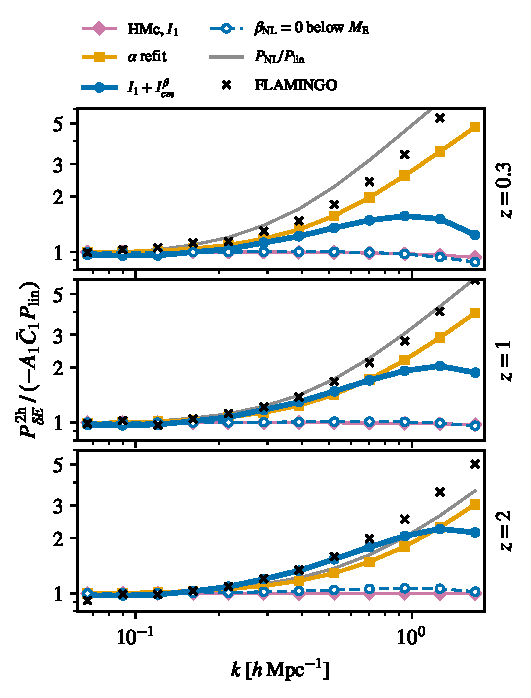
\includegraphics[width=3.5in]{plots/gi_kernel/gi_kernel.pdf}
  \caption{The 2-halo GI spectrum per unit $-A_1\Cb\Plin$ at $z = 0.3$, 1
  and 2: HMc ($I_1$, purple diamonds), the $\alpha$ model at its FLAMINGO
  best fit (orange squares), $\bNL$ (thick blue circles), $\bNL$ set to 0
  below the emulator's masses (dashed, open circles), $\PNL/\Plin$ (gray) and
  FLAMINGO's $P_{\delta E}$ (crosses).}
  \label{fig:kernel}
\end{figure}

\paragraph{How a halo model enters Roman.} Cosmolike computes native NLA or
TATT. A halo model differs from it only in $S_{\rm GI}$ and $S_{\rm II}$, so
its data vector is the native one plus a template, exact in the IA
amplitudes:
\begin{equation}
\Delta\xi = \sum_s\Big[A_sU^{\rm GI}_s + A_s^2U^{\rm II}_s\Big],\quad
U^{\rm GI}_s = \sum_jR^{\rm GI}_{sj}\,\frac{\Cb(z_s)\,[1 - S_{\rm GI}/\PNL](k_j,z_s)}{R_{\delta E}(k_j,z_s)},
\end{equation}
and $U^{\rm II}_s$ the same with $-\Cb^2[1 - S_{\rm II}/\PNL]/R_{EE}$, where
$A_s = A_1[(1+z_s)/1.62]^{\eta_1}$, $R^X_{sj}$ is the response of the data
vector to the truth's $P_X$ on the $\ln k$ tent $j$ at snapshot $s$, and
$R_X$ the truth's ratio to $\PNL$
(\texttt{analysis/cut\_validation/hm\_templates.py}). The templates are held
at the fiducial cosmology. For CP the II template uses the $E$ part of the
base, since no model changes the $B$ modes. The fitted models are TATTh and
NLAh (HMc), TATTa and NLAa ($\alpha$ free), TATTf and NLAf ($\alpha$ of
FLAMINGO), and TATTb and NLAb ($\bNL$).

\section{Goodness of fit on FLAMINGO}
\label{sec:gof}

In the TATT form, only the $\alpha$ model fits FLAMINGO beyond
$\kmax \approx 0.5$ (Fig.~\ref{fig:gof}). At $\kmax = 0.52$ the summed
$\chi^2/\nu$ is \gofTattBaseA\ for TATT on $\PNL$, \gofTattHmcA\ for HMc,
\gofTattNlbA\ for $\bNL$ and \gofTattAlphaA\ for $\alpha$. At $\kmax = 0.94$
it is \gofTattBaseC, \gofTattHmcC, \gofTattNlbC\ and \gofTattAlphaC. $\bNL$ is
the best physical model to $\kmax = 0.70$ and worse than HMc from 0.94 on,
where its turnover (Fig.~\ref{fig:kernel}) takes away power that HMc's
$\bTA$ can still supply. The goodness-of-fit cuts are
\cutTattBaseLo\ to \cutTattBaseHi$\hMpc$ (TATT), \cutTattHmcLo\ to
\cutTattHmcHi\ (HMc), \cutTattNlbLo\ to \cutTattNlbHi\ ($\bNL$) and
\cutTattAlphaLo\ to \cutTattAlphaHi\ ($\alpha$).

In the NLA form every model is worse, since $\bTA$ is no longer there to take
up the missing power. HMc in the NLA form fails at every $\kmax$
(\gofNlaHmcA\ at 0.52); $\bNL$ is \gofNlaNlbA, NLA \gofNlaBaseA\ and $\alpha$
\gofNlaAlphaA. The NLA-form $\alpha$ model has cuts of \cutNlaAlphaLo\ to
\cutNlaAlphaHi$\hMpc$.

\begin{figure}[t]
  \centering
  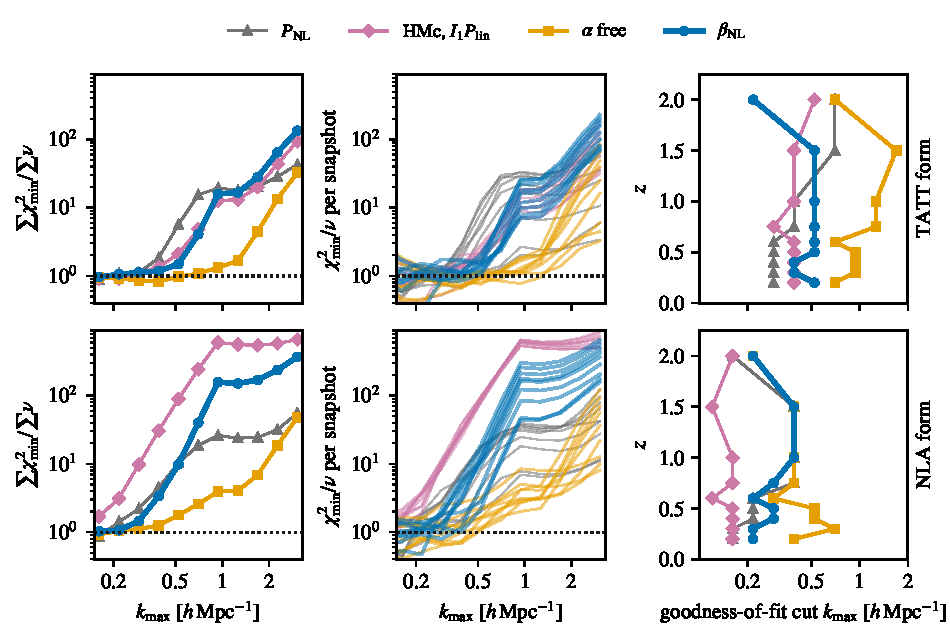
\includegraphics[width=\textwidth]{plots/gof/gof.pdf}
  \caption{Goodness of fit to FLAMINGO's $P_{hE}$, $P_{EE}$ and $P_{BB}$
  at the nine core snapshots. Top row: TATT form ($A_2$, $\bTA$ free);
  bottom row: NLA form. Left: summed $\chi^2_{\min}/\nu$ against $\kmax$;
  middle: $\chi^2_{\min}/\nu$ per snapshot (thin); right: the goodness-of-fit
  cut per snapshot redshift. $A_1$ terms on $\PNL$ (gray triangles), on
  $I_1\Plin$ (HMc, purple diamonds), with $\alpha$ free (orange squares) and
  with $\bNL$ (thick blue circles). Dotted: $\chi^2/\nu = 1$.}
  \label{fig:gof}
\end{figure}

\section{Physical checks}
\label{sec:checks}

\paragraph{Failed: the central 1-halo amplitude sits at its cap.} At
$\kmax = 0.52$, $a_c = 1$ at \acCapTattHmcA\ of 9 snapshots for HMc,
\acCapTattNlbA\ for $\bNL$ and \acCapTattAlphaA\ for $\alpha$ (TATT form;
\acCapTattBaseA\ for TATT on $\PNL$). The term takes all the power it is
allowed (Fig.~\ref{fig:params}, third row). With $a_c$ free, HMc needed
$a_c = 13$ to 190 (HMc review): the cap hides the problem, it does not solve
it.

\paragraph{Failed: $\bTA$ absorbs the 2-halo deficit in HMc and $\bNL$.} It
rises with the fit range, from \btaHmcALo\ to \btaHmcAHi\ at $\kmax = 0.52$ to
\btaHmcCLo\ to \btaHmcCHi\ at 0.94 for HMc, and from \btaNlbALo\ to
\btaNlbAHi\ to \btaNlbCLo\ to \btaNlbCHi\ for $\bNL$. In the $\alpha$ model it
stays between \btaAlphaALo\ and \btaAlphaAHi\ and does not grow. A density
weighting that grows with $\kmax$ is the missing nonlinear power, not a
density weighting.

\paragraph{Failed in the NLA form: $\alpha$ exceeds 1.} The NLA-form $\alpha$
is \alphaNlaALo\ to \alphaNlaAHi\ at $\kmax = 0.52$, above its physical range at
$z \ge 1.5$, because without $\bTA$ it is the only parameter that can add
power. In the TATT form it is \alphaTattALo\ to \alphaTattAHi\ (0.52) and
\alphaTattCLo\ to \alphaTattCHi\ (0.94), inside 0 to 1 and stable, but it
rises with redshift and is anticorrelated with $\bTA$.

\paragraph{Mixed: $A_1$ is stable in the $\alpha$ model and drifts elsewhere.}
The ratio $A_1(\kmax = 0.94)/A_1(0.29)$ over the snapshots is
\driftTattAlphaLo\ to \driftTattAlphaHi\ for $\alpha$, \driftTattNlbLo\ to
\driftTattNlbHi\ for $\bNL$ and \driftTattHmcLo\ to \driftTattHmcHi\ for HMc
(TATT form). In the NLA form HMc's $A_1$ rises by a factor \driftNlaHmcLo\ to
\driftNlaHmcHi\ and $\bNL$'s by \driftNlaNlbLo\ to \driftNlaNlbHi.

\paragraph{Passed: the low-$k$ limit.} Every model reduces to NLA (or TATT)
below $k \approx 0.1$. At $\kmax = 0.29$ the fitted $A_1$ of the four models
agree to \lowkSpreadTattLo\ to \lowkSpreadTattHi\% per snapshot (TATT form)
and \lowkSpreadNlaLo\ to \lowkSpreadNlaHi\% (NLA form): the models already
differ at $k = 0.2$ to 0.3.

\begin{figure}[t]
  \centering
  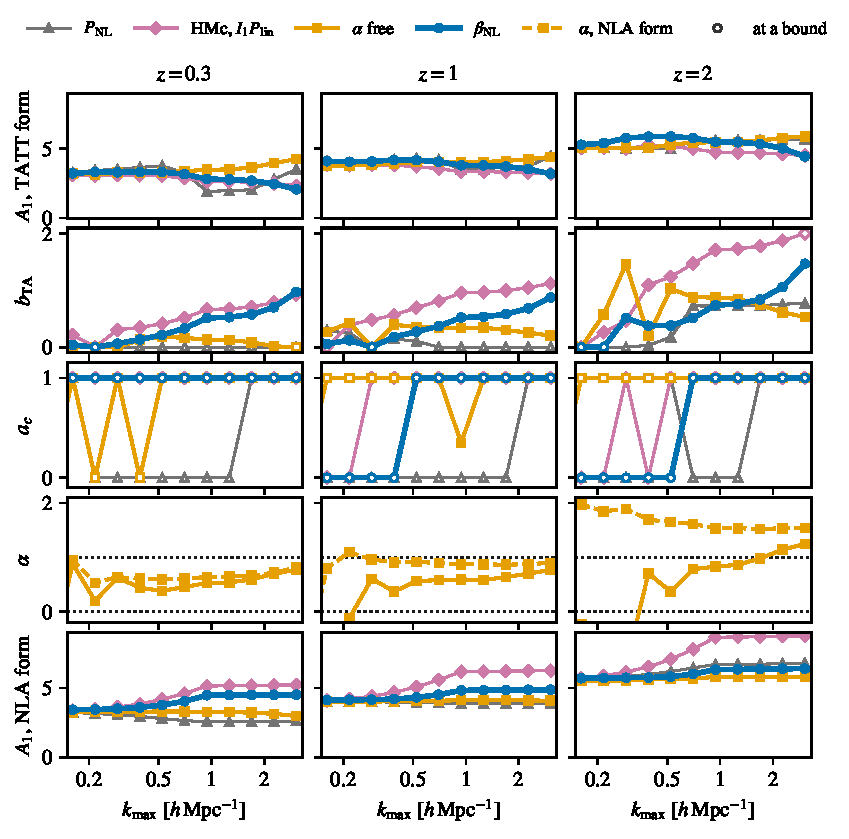
\includegraphics[width=\textwidth]{plots/params/params.pdf}
  \caption{Best-fit parameters against $\kmax$ at $z = 0.3$, 1 and 2. Rows:
  $A_1$, $\bTA$ and $a_c$ of the TATT form; $\alpha$ of the $\alpha$ model
  (TATT form solid, NLA form dashed); $A_1$ of the NLA form. Models encoded as
  in Fig.~\ref{fig:gof}. Open markers: the parameter is within 1\% of a
  bound. Dotted: $a_c = 1$ and $\alpha = 0$, 1. Below
  $\kmax \approx 0.3$, $\alpha$ and $a_c$ are not constrained.}
  \label{fig:params}
\end{figure}

\section{Figure of bias for Roman}
\label{sec:fob}

Figure~\ref{fig:fob} shows the FoB of every model against the $\xi_\pm$ cut.
The quantity that sets a cut is the largest $K_0$ up to which the FoB stays
below 0.3:

\begin{center}\footnotesize
\begin{tabular}{lccccc}
\toprule
probe, form & $\PNL$ & HMc & $\alpha$ free & $\alpha$ of FLAMINGO & $\bNL$ \\
\midrule
shear, TATT & \kmaxCsTattBase & \kmaxCsTattHmc & \kmaxCsTattAlpha & \kmaxCsTattAlphaf & \kmaxCsTattNlb \\
shear, NLA & \kmaxCsNlaBase & \kmaxCsNlaHmc & \kmaxCsNlaAlpha & \kmaxCsNlaAlphaf & \kmaxCsNlaNlb \\
3x2pt, TATT & \kmaxTxTattBase & \kmaxTxTattHmc & \kmaxTxTattAlpha & \kmaxTxTattAlphaf & \kmaxTxTattNlb \\
3x2pt, NLA & \kmaxTxNlaBase & \kmaxTxNlaHmc & \kmaxTxNlaAlpha & \kmaxTxNlaAlphaf & \kmaxTxNlaNlb \\
\bottomrule
\end{tabular}
\end{center}

\paragraph{The $\alpha$ models follow NLA and TATT.} Roman does not measure
$\alpha$, and with $\alpha$ free the FoB stays within 0.05 of the native model
at every cut, as it did on the S1 truth. Holding $\alpha$ at FLAMINGO's value
raises the FoB slightly (\fobTopCsTattAlphaf\ against \fobTopCsTattBase\ at
$K_0 = 0.6$ in cosmic shear, TATT form).

\paragraph{HMc in the TATT form is more biased.} In cosmic shear its FoB is
\fobCsTattHmc\ at $K_0 = 0.35$ against \fobCsTattBase\ for TATT, and
\fobTopCsTattHmc\ at 0.6, so its cut tightens to \kmaxCsTattHmc. Its reference
fit is worse at every cut from $K_0 = 0.25$ on ($\chi^2 = \ctwoTopCsTattHmc$ against
\ctwoTopCsTattBase\ at 0.6).

\paragraph{HMc in the NLA form is less biased, for the wrong reason.} In
3x2pt its FoB stays below 0.3 at every $K_0$ (\fobTopTxNlaHmc\ at 0.6 against
\fobTopTxNlaBase\ for NLA). But its reference $\chi^2$ is \ctwoTopTxNlaHmc\
against \ctwoTopTxNlaBase\ at 0.6 (\ctwoTopCsNlaHmc\ against
\ctwoTopCsNlaBase\ in cosmic shear), and it is the worst fit to FLAMINGO of all
models (section ``Goodness of fit on FLAMINGO''). Its missing power at
$k \gtrsim 0.2$ shifts the IA fit in a direction that happens to cancel part of
the cosmology shift. Nothing in the model ties this cancellation to
another truth.

\paragraph{$\bNL$ depends on the form.} In the TATT form it is the least
biased model in cosmic shear at every cut from $K_0 = 0.25$ on (\fobCsTattNlb\ at $K_0 = 0.35$,
\fobTopCsTattNlb\ at 0.6) and in 3x2pt below $K_0 = 0.3$, with a reference
$\chi^2$ close to TATT's (\ctwoTopCsTattNlb\ against \ctwoTopCsTattBase\ at
0.6). Its $\bTA$ sits at 0 and its $\eta_2$ at a bound in the reference fit at
some cuts, as native TATT's do. The cuts do not move: cosmic shear stays at
\kmaxCsTattNlb, 3x2pt at \kmaxTxTattNlb. In the NLA form $\bNL$ is the most
biased model in cosmic shear (\fobTopCsNlaNlb\ at 0.6; cut \kmaxCsNlaNlb\
against \kmaxCsNlaBase), and less biased than NLA in 3x2pt (cut
\kmaxTxNlaNlb\ against \kmaxTxNlaBase), again with a worse reference fit
(\ctwoTopTxNlaNlb\ against \ctwoTopTxNlaBase).

\paragraph{Why the differences are small in the TATT form.} Roman's $\xi_\pm$
at these cuts weights $k \lesssim K_0/D(z)$, where the models differ by tens
of percent at most (Fig.~\ref{fig:kernel}), and $A_1$, $\eta_1$, $A_2$ and
$\bTA$ absorb most of that difference. Without $A_2$ and $\bTA$ (NLA form) the
same difference moves the cosmology, which is why the NLA-form FoB spreads
from below 0.1 to above 0.6.

\begin{figure}[t]
  \centering
  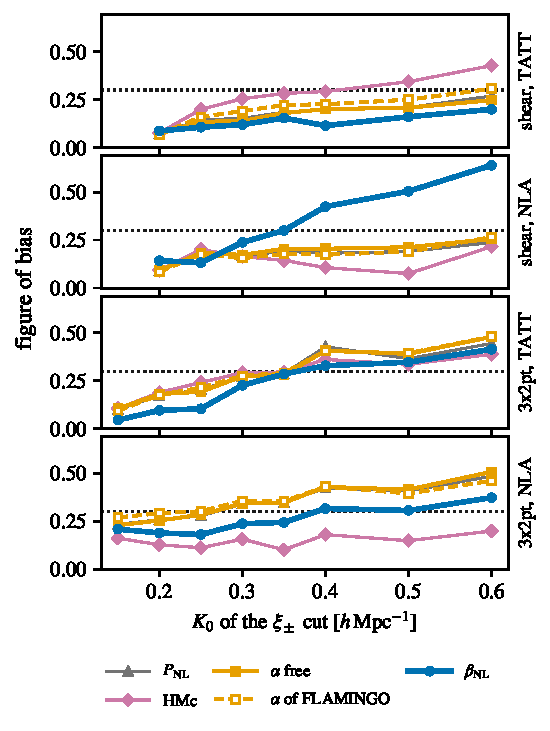
\includegraphics[width=3.5in]{plots/fob_k0scan/fob_k0scan.pdf}
  \caption{Roman's 2D figure of bias against the $\xi_\pm$ cut $K_0$, CP
  truth, every parameter free with the CMB prior, Fisher shift. Panels: cosmic
  shear and 3x2pt ($\gamma_t$ at 0.5, $w$ at 0.2), each in the TATT and the
  NLA form. $A_1$ terms on $\PNL$ (gray triangles), HMc (purple diamonds),
  $\alpha$ free (orange squares), $\alpha$ of FLAMINGO (orange, dashed, open
  squares) and $\bNL$ (thick blue circles). Dotted: 0.3.}
  \label{fig:fob}
\end{figure}

\appendix

\section{Numerical checks}
\label{app:checks}

\begin{itemize}
\item The $\bNL$ tables and the FLAMINGO fits were rerun on this Mac from
  scratch. They reproduce the cloud run of 24 November 2026 to $10^{-3}$
  ($\Plin$, CAMB 1.6.7 against the stored v6 tables) and the summed
  $\chi^2/\nu$ to $10^{-3}$.
\item The $\alpha$-model fits reproduce the HMc review's refit (summed
  $\chi^2/\nu$ \gofTattAlphaA, \gofTattAlphaB, \gofTattAlphaC\ at
  $\kmax = 0.52$, 0.70, 0.94), and TATT on $\PNL$ reproduces its TATT $+ W$
  reference to 7\%; the difference is the $a_c$ term, which the reference
  did not have.
\item The \Nsnap-snapshot $\bNL$ integrals for Roman reproduce the
  nine-snapshot tables of the fits exactly at the core snapshots.
\item The CP templates rebuild cosmolike's native NLA from the same
  template sum to $\Delta\chi^2 = 0.009$ (cosmic shear) and 0.010 (3x2pt) at
  $A_1 = 3.5$, $\eta_1 = 0.7$ (\texttt{fisher\_minimize.py --check-hm CP}),
  as the earlier templates did. The S1 templates were regenerated
  bit-identical.
\end{itemize}

\section{Where the code and results are}
\label{app:code}

\begin{center}\footnotesize
\begin{tabular}{lll}
\toprule
result & folder & script $\rightarrow$ output \\
\midrule
$\bNL$ tables, 9 snapshots & \texttt{analysis/halo\_nlbias} & \texttt{beta\_tables.py} $\rightarrow$ \texttt{beta\_tables.npz} \\
$\bNL$ integrals & same & \texttt{halo\_nlbias.py} $\rightarrow$ \texttt{nlbias\_tables.npz} \\
the same, 13 snapshots & same & \texttt{nlbias\_roman\_tables.py} $\rightarrow$ \texttt{nlbias\_roman\_tables.npz} \\
FLAMINGO fits & same & \texttt{nlbias\_fit.py} $\rightarrow$ \texttt{nlbias\_fits.json} \\
Roman templates & \texttt{analysis/cut\_validation} & \texttt{hm\_templates.py S1 CP} \\
Roman FoB & same & \texttt{run\_fisher\_jobs.sh jobs\_halo\_cp.txt 4} \\
figures, numbers & \texttt{notes/halo\_ia\_models} & \texttt{plots/make\_figure\_data.py}, \texttt{make\_numbers.py} \\
\bottomrule
\end{tabular}
\end{center}

Dark Emulator runs in its own environment, \texttt{\~{}/cocoa/venvs/darkemu},
with CAMB taken from the cocoa environment (\texttt{PYTHONPATH} set to its
\texttt{site-packages}). The cosmolike runs use the cocoa environment.

\section{Open issues}
\label{app:open}

\begin{itemize}
\item $\bNL$ below $10^{\lgMEhi}\Msun$ is an extrapolation, and most centrals
  live there. A $\bNL$ measured from FLAMINGO's own halo catalogues per mass
  bin would test the held value directly.
\item The model with physics in the 1-halo regime is still missing. Neither
  1-halo term has the scale dependence FLAMINGO needs. Populating FLAMINGO's
  halos with aligned galaxies (Van Alfen et al.\ 2023, arXiv:2311.07374)
  avoids the analytic transition.
\item $\bNL$ at $z = 3$ and 4 uses a peak-height assignment from
  $z = \ZEmu$; those snapshots carry little weight in Roman's kernels.
\item The FoB is the Fisher shift on one truth; minimizer runs and other
  truths were not run for these models.
\end{itemize}

\end{document}
